%!TEX root = ../thesis.tex
%*******************************************************************************
%****************************** Second Chapter *********************************
%*******************************************************************************
\chapter{Data Quality Dimensions}

\ifpdf
    \graphicspath{{Chapter2/Figs/Raster/}{Chapter2/Figs/PDF/}{Chapter2/Figs/}}
\else
    \graphicspath{{Chapter2/Figs/Vector/}{Chapter2/Figs/}}
\fi


More specifically, quality dimensions can refer either to the extension of data, i.e., to data values, or to their 
intension, i.e., to their schema. Both data dimensions are usually defined in qualitative way, referring to general properties of data and schemas,
and and related definitions do not provide any facility for assigning values to dimensions themselves. 

Specifically, definitions do not provide quantitative measures, and one or more metrics are to be associated with dimensions as separate, distinct 
properties. For each metric, one or more measurement methods are to be provided regarding (i) where the measurement is taken, (ii) what data are included, 
(iii) the measurement device, and (iv) the scale on which results are reported.

According to the literature, at times we will distinguish between dimensions and metrics, while other times we will directly metrics.

\begin{table}[H]
\caption{Data Quality Dimensions I}
\centering
\begin{tabular}{p{4.0cm} p{10cm}}
\toprule
\textbf{Dimension Name} & \textbf{Description} \\ 
\bottomrule
Data Governance & 
Do organization-wide data standards exist and are they enforced? Do clearly
defined roles and responsibilities exist for data quality related activities? Does
data governance strive to acquire and maintain high-quality data through proactive
management? \\
Data Specifications &
Are data standards documented in the form of a data dictionary, 
data models, meta data, and integrity constraints?  
\\
Data Integrity & 
How is data integrity maintained? How are data integrity violations detected and
resolved ?   
\\
Data Consistency & 
If data redundancy exists, how is data consistency achieved? What methods
are used to bring consistency to data that has become inconsistent? If data is
geographically replicated, how is the consistency and latency managed? 
\\
Data Currency & 
Is the data current? Do procedures exists to keep the data current and purge stale
data? 
\\
Data Duplication & Are there effective procedures in place to detect and remove duplicate data? 
\\
Data Completeness & 
Is the data about entities complete? How is missing data managed? 
\\
Data Provenance & 
Is a historical record of data and its origination maintained? If the data is acquired
through multiple sources and has undergone cleaning and transformations, does
the organization maintain a history of all changes to the data? 
\\
Data Heterogeneity & 
If multi-modality data about an entity is available, is that data captured and used? 
\\
Streaming Data & 
How is streaming data sampled, filtered, stored, and managed for both real-time
and batch processing? 
\\
Outliers & 
How are outliers detected and addressed? Are there versions of datasets that
are outlier-free? Does each version correspond to a different method for outlier
detection and treatment? 
\\
Dimensionality &
Reduction Do the datasets feature dimensionality reduced versions? How many versions are
available? \\
Feature Selection & 
Do datasets have versions that exclude features that are either redundant, highly
correlated, or irrelevant? How many versions are available? 
\\
\bottomrule
\end{tabular}
\end{table}

\begin{table}
% \vspace*{-3.5in}
\caption{Data Quality Dimensions II}
\centering
\begin{tabular}{p{4.0cm} p{10cm}}
\toprule
\textbf{Dimension Name} & \textbf{Description} \\ 
\bottomrule
Feature Extraction & 
Do the datasets provide a set of derived features that are informative and non-
redundant, in addition to the original set of variables/features? How many such
derived feature sets are available? 
\\
Business Rules & 
Does a process exist to identify, refine, consolidate, and maintain business
rules that pertain to data quality? Do rules exist to govern data cleaning and
transformations, and integrating related data of an entity from multiple sources?
What business rules govern substitutions for missing data, deleting duplicate data,
and archiving historical data? Are there rules for internal data audit and regulatory
compliance? \\
Data Accuracy & 
Data can be syntactically accurate and yet semantically inaccurate. For example,
a customer's mailing address may meet all the syntactic patterns specified by the
postal service, yet it can be inaccurate. How does the organization establish the
accuracy of data? \\
Gender Bias & 
Is the data free from factors that lead to gender bias in machine learning
algorithms? \\
Confidentiality and Privacy & 
Are procedures and controls implemented for data encryption, data de-
identification and re-identification, and differential privacy? \\
Availability and Access Controls & 
How is high data availability achieved? What security controls are implemented to
protect data from unauthorized access? How are user entitlements to data access
and modifications defined and implemented? \\
\bottomrule
\end{tabular}
\end{table}


\section{Accuracy}

Accuracy ~\citep{Falorsi} is defined as the closeness between a value v and a value v' , considered as 
the correct representation of the real-life phenomenon that v aims to
represent. As an example if the name of a person is John, the value v' = Aytaç
is correct, while the value v = Ayt is incorrect. Two kinds of accuracy can be
identified, namely a syntactic accuracy and a semantic accuracy.

Let us consider a relation schema \textbf{R} consisting of \textbf{K}
attributes and a relational table \textbf{r} consisting of N tuples. 

Let $q_{ij}(i=1..N, j=1..K)$ be a boolean variable defined to correspond to the cell values 
$y_{ij}$, is syntactically accurate, while otherwise it is equal to 1. 

In order to identify whether or not accuracy errors affect a matching of 
relational table \textbf{r} with a reference table \textbf{r'} containing correct
values, we introduce a further boolean variable $s_i$ equal to 0 if the tuple $t_i$ 
matches a tuple in \textbf{r'}, and otherwise equal to 1. We can introduce three metrics to distinguish
the relative importance of value accuracy in context of the tuple.
The first two metrics have the purpose of giving a different importance to 
errors on attributes that have a higher identification power, in line with 
the above discussion.

The first metric called \textit{weak accuracy error,} and is defined:

\begin{equation*}
    \sum_{i = 1}^{N} \frac{\beta(q_i > 0)\wedge(s_i=0)}{N}
\end{equation*}

where $\beta(.)$ is a boolean variable equal to 1 if the condition in parentheses is 
\textit{true}, 0 otherwise, and $q_i =\sum\nolimits_{j=1}^K q_{ij}$. Such metric considers the case in 
which for a tuple $t_i$ accuracy errors occur $(q_i > 0)$ but do not affect identification
$(s_i = 0)$.

The second metric is called \textit{strong accuracy error}, and is defined assigning

\begin{equation*}
    \sum_{i = 1}^{N} \frac{\beta(q_i > 0)\wedge(s_i=1)}{N}
\end{equation*}

where $\beta(.)$ and $q_i$ have the same meaning as above. Such a metric considers
the case which accuracy errors occur $(q_i > 0)$ for a tuple $t_i$ and actually 
do affect identification $(s_i = 1)$.

The third metric gives the percentage of accurate tuples matched with
the reference table. It is expressed by the degree of syntactic accuracy of the
relational instance \textbf{r}

\begin{equation*}
    \sum_{i = 1}^{N} \frac{\beta(q_i =0)\wedge(s_i=0)}{N}
\end{equation*}

by actually considering the fraction of accurate $(q_i = 0)$ matched $(s_i =0)$ tuples.

\section{Completeness}
Completeness can be generically defined as the extent to which data are
of sufficient breadth, depth, and scope for the task at hand ~\cite{Wang}
three types of completeness are identified. Schema completeness is defined as
the degree to which concepts and their properties are not missing from the
schema. Column completeness is defined as a measure of the missing values for
a specific property or column in a table. Population completeness evaluates
missing values with respect to a reference population.
If focusing on a specific data model, a more precise characterization of
completeness can be given. In the following we refer to the relational model.

\subsection{Completeness of Web Data}

Data that are published in Web information systems can be characterized by
evolution in time. While in the traditional paper-based media, information
is published once and for all, Web information systems are characterized by
information that is continuously published.

We consider a function $C(t)$, defined as the value of completeness at the
instant \textit{t}, with $t\in$ $[t\_pub, t\_max]$ , where t pub is the initial 
instant of publication of data and ${t\_max}$ corresponds to the maximum time within which the
series of the different scheduled updates will be completed. Starting from the
function $C(t)$, we can define the completability of the published data as

\begin{equation*}
    \int\nolimits_{t\_curr}^{t\_max} C(t),
\end{equation*}

where ${t\_curr}$ is the time at which completability is evaluated and ${t\_curr}$ <
${t\_max}$.

Completability, as shown in Figure 2.1, can be graphically depicted as an
area Cb of a function that represents how completeness evolves between an
instant ${t\_curr}$ of observation and t max. Observe that the value corresponding
to ${t\_curr}$ is indicated as ${c\_curr}$; ${c\_max}$ is the value for completeness estimated
for t max. The value ${c\_max}$ is a real reachable limit that can be specified for
the completeness of the series of elements; if this real limit does not exist,
${c\_max}$ is equal to 1. In Figure 2.5, a reference area A is also shown, defined as

\begin{equation*}
    ({t\_max}-{t\_curr}) * \frac{{c\_max - {c\_pub}}}{2},
\end{equation*}

that, by comparison with Cb, allows us to define ranges [High, Medium, Low]
for completability.

\begin{figure}[H]
    \vspace*{.0in}
    \centering
    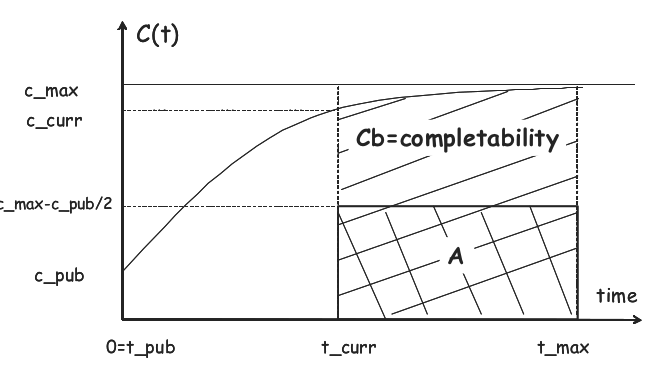
\includegraphics[scale=.50]{completeness_of_web_data}
    \caption{A graphical representation of completability}    
\end{figure}

With respect to the example above, considering the list of courses published on a university Web site, the completeness dimension gives information
about the current degree of completeness; the completability information gives
the information about how fast this degree will grow in time, i.e., how fast
the list of courses will be completed. The interested reader can find further
details in ~\cite{pernicib.scannapiecom.2003}.

\section{Consistency}

The consistency dimension captures the violation of semantic rules defined
over (a set of) data items, where items can be tuples of relational tables or
records in a file. With reference to relational theory, integrity constraints are
an instantiation of such semantic rules. In statistics, data edits are another
example of semantic rules that allow for the checking of consistency.

\subsection{Integrity Constraints}
Integrity constraints are properties that must be satisfied by all instances
of a database schema. Although integrity constraints are typically defined on
schemas, they can at the same time be checked on a specific instance of the
schema that presently represents the extension of the database. Therefore,
we may define integrity constraints for schemas, describing a schema quality
dimension, and for instances, representing a data dimension.

Most of the considered integrity constraints are dependencies. The follow-
ing main types of dependencies can be considered:

\begin{itemize}
    \item{\textit{Key Dependency.} This is the simplest type of dependency. Given a relation
    instance r, defined over a set of attributes, we say that for a subset K of
    the attributes a key dependency holds in r, if no two rows of r have the
    same K-values. For instance, an attribute like SocialSecurityNumber can
    serve as a key in any relation instance of a relation schema Person.}
    \item{\textit{Inclusion Dependency.} Inclusion dependency is a very common type of
    constraint, and is also known as referential constraint. An inclusion de-
    pendency over a relational instance r states that some columns of r are
    contained in other columns of r or in the instances of another relational in-
    stance s. A foreign key constraint is an example of inclusion dependency,
    stating that the referring columns in one relation must be contained in the
    primary key columns of the referenced relation.}
    \item{\textit{Functional Dependency.} Given a relational instance \textbf{r}, let \textbf{X} and \textbf{Y} be two
    nonempty sets of attributes in \textbf{r}. \textbf{r} satisfies the functional dependency
    ${\textbf{X} \rightarrow \textbf{Y}}$ if the following holds for every pair of tuples \textbf{$t_1$} and \textbf{$t_2$} in \textbf{r}:
    }
\end{itemize}

\begin{equation*}
    \boxed{If, t_1.X = t_2.X, then, t_1.Y = t_2.Y,}
\end{equation*}

where the notation $t_1.X$ means the projection of the tuple $t_1$ onto the
attributes in $X$.

\section{Other Data Quality Dimensions}